\def\bmode{0} % Mode 0 for presentation, mode 1 for a handout with notes, mode 2 fo% r handout without notes
\if 0\bmode
\documentclass[usenames,dvipsnames,smaller, hyperref={colorlinks=true,urlcolor=magenta,citecolor=cyan,linkcolor=orange}]{beamer}
\else \if 1\bmode
\immediate\write18{pdflatex -jobname=\jobname-Handout-Notes\space\jobname}
\documentclass[usenames,dvipsnames,smaller,handout,hyperref={colorlinks=true,urlcolor=magenta,citecolor=cyan,linkcolor=orange}]{beamer}
\usepackage{handoutWithNotes}
\pgfpagesuselayout{2 on 1 with notes}[letterpaper, landscape, border shrink=4mm]
\else \if 2\bmode
\immediate\write18{pdflatex -jobname=\jobname-Handout\space\jobname}
\documentclass[usenames,dvipsnames,smaller,handout,hyperref={colorlinks=true,urlcolor=magenta,citecolor=cyan,linkcolor=orange}]{beamer}
\fi
\fi
\fi

% \documentclass[smaller,handout
% ]{beamer}
%\usepackage{etex}
%\newcommand{\num}{6{} }

% \usetheme[
%   outer/progressbar=foot,
%   outer/numbering=counter,
%  block=fill
% ]{metropolis}

%\useoutertheme{metropolis}

\usetheme{Madrid}
\useoutertheme[subsection=false]{miniframes} % Alternatively: miniframes, infolines, split
\useinnertheme{circles}
\usecolortheme{seahorse}

\usepackage[backend=biber,style=authoryear,maxcitenames=2,maxbibnames=99,safeinputenc,url=false,
eprint=false]{biblatex}
\addbibresource{bib/references.bib}
\AtEveryCitekey{\iffootnote{{\tiny}\tiny}{\tiny}}

%\usepackage{pgfpages}
%\setbeameroption{hide notes} % Only slides
%\setbeameroption{show only notes} % Only notes
%\setbeameroption{hide notes} % Only notes
%\setbeameroption{show notes on second screen=right} % Both

% \usepackage[sfdefault]{Fira Sans}

% \setsansfont[BoldFont={Fira Sans}]{Fira Sans Light}
% \setmonofont{Fira Mono}

%\usepackage{fira}
%\setsansfont{Fira}
%\setmonofont{Fira Mono}
% To give a presentation with the Skim reader (http://skim-app.sourceforge.net) on OSX so
% that you see the notes on your laptop and the slides on the projector, do the following:
% 
% 1. Generate just the presentation (hide notes) and save to slides.pdf
% 2. Generate onlt the notes (show only nodes) and save to notes.pdf
% 3. With Skim open both slides.pdf and notes.pdf
% 4. Click on slides.pdf to bring it to front.
% 5. In Skim, under "View -> Presentation Option -> Synhcronized Noted Document"
%    select notes.pdf.
% 6. Now as you move around in slides.pdf the notes.pdf file will follow you.
% 7. Arrange windows so that notes.pdf is in full screen mode on your laptop
%    and slides.pdf is in presentation mode on the projector.

% Give a slight yellow tint to the notes page
%\setbeamertemplate{note page}{\pagecolor{yellow!5}\insertnote}\usepackage{palatino}


%\usetheme{metropolis}
%\usecolortheme{beaver}
%\usepackage{xcolor}
\definecolor{darkcandyapplered}{HTML}{A40000}
\definecolor{lightcandyapplered}{HTML}{e74c3c}

%\setbeamercolor{title}{fg=darkcandyapplered}
%\setbeamercolor{frametitle}{bg=darkcandyapplered!80!black!90!white}
%\setbeamertemplate{frametitle}{\bf\insertframetitle}
%\setbeamercolor{footnote mark}{fg=darkcandyapplered}
%\setbeamercolor{footnote}{fg=darkcandyapplered!70}
%\Raggedbottom
%\setbeamerfont{page number in head/foot}{size=\tiny}
%\usepackage[tracking]{microtype}


\setbeamertemplate{frametitle}{%
    \nointerlineskip%
    \begin{beamercolorbox}[wd=\paperwidth,ht=2.0ex,dp=0.6ex]{frametitle}
        \hspace*{1ex}\insertframetitle%
    \end{beamercolorbox}%
}



\setbeamerfont{caption}{size=\footnotesize}
\setbeamercolor{caption name}{fg=darkcandyapplered}


%\usepackage[sc,osf]{mathpazo}   % With old-style figures and real smallcaps.
%\linespread{1.025}              % Palatino leads a little more leading

% Euler for math and numbers
%\usepackage[euler-digits,small]{eulervm}
%\AtBeginDocument{\renewcommand{\hbar}{\hslash}}
\usepackage{graphicx,multirow,paralist,booktabs}


%\mode<presentation> { \setbeamercovered{transparent} }

\setbeamertemplate{navigation symbols}{}
\makeatletter
\def\beamerorig@set@color{%
  \pdfliteral{\current@color}%
  \aftergroup\reset@color
}
\def\beamerorig@reset@color{\pdfliteral{\current@color}}
\makeatother

%=== GRAPHICS PATH ===========
\graphicspath{{./m2-images/}}
% Marginpar width
%Marginpar width
%\setlength{\marginparsep}{.02in}


%% Captions
% \usepackage{caption}
% \captionsetup{
%   labelsep=quad,
%   justification=raggedright,
%   labelfont=sc
% }

%AMS-TeX packages

\usepackage{amssymb,amsmath,amsthm} 
\usepackage{bm}
\usepackage{color}

\usepackage{hyperref,enumerate}
\usepackage{minitoc,array}


%https://tex.stackexchange.com/a/31370/2269
\usepackage{mathtools,cancel}

\renewcommand{\CancelColor}{\color{red}} %change cancel color to red

\makeatletter
\let\my@cancelto\cancelto %copy over the original cancelto command
\newcommand<>{\cancelto}[2]{\alt#3{\my@cancelto{#1}{#2}}{\mathrlap{#2}\phantom{\my@cancelto{#1}{#2}}}}
% redefine the cancelto command, using \phantom to assure that the
% result doesn't wiggle up and down with and without the arrow
\makeatother


\definecolor{slblue}{rgb}{0,.3,.62}
\hypersetup{
    colorlinks,%
    citecolor=blue,%
    filecolor=blue,%
    linkcolor=blue,
    urlcolor=slblue
}

%%%TIKZ
\usepackage{tikz}
\usepackage{pgfplots}
\usepackage{pgfplotstable}
\usepackage{pgfgantt}
\usepackage{tikzsymbols}
\pgfplotsset{compat=newest}

\usetikzlibrary{arrows,shapes,positioning,shapes.geometric}
\usetikzlibrary{decorations.markings}
\usetikzlibrary{shadows,automata}
\usetikzlibrary{patterns}
\usetikzlibrary{trees,mindmap,backgrounds}
%\usetikzlibrary{circuits.ee.IEC}
\usetikzlibrary{decorations.text}
% For Sagnac Picture
\usetikzlibrary{%
    decorations.pathreplacing,%
    decorations.pathmorphing%
}
\tikzset{no shadows/.style={general shadow/.style=}}
%
%\usepackage{paralist}


%%% FORMAT PYTHON CODE
%\usepackage{listings}
% Default fixed font does not support bold face
\DeclareFixedFont{\ttb}{T1}{txtt}{bx}{n}{8} % for bold
\DeclareFixedFont{\ttm}{T1}{txtt}{m}{n}{8}  % for normal

% Custom colors
\definecolor{deepblue}{rgb}{0,0,0.5}
\definecolor{deepred}{rgb}{0.6,0,0}
\definecolor{deepgreen}{rgb}{0,0.5,0}

%\usepackage{listings}

% Python style for highlighting
% \newcommand\pythonstyle{\lstset{
% language=Python,
% basicstyle=\footnotesize\ttm,
% otherkeywords={self},             % Add keywords here
% keywordstyle=\footnotesize\ttb\color{deepblue},
% emph={MyClass,__init__},          % Custom highlighting
% emphstyle=\footnotesize\ttb\color{deepred},    % Custom highlighting style
% stringstyle=\color{deepgreen},
% frame=tb,                         % Any extra options here
    % showstringspaces=false            % 
% }}

% % Python environment
% \lstnewenvironment{python}[1][]
% {
% \pythonstyle
% \lstset{#1}
% }
% {}

% % Python for external files
% \newcommand\pythonexternal[2][]{{
% \pythonstyle
% \lstinputlisting[#1]{#2}}}

% Python for inline
% 
% \newcommand\pythoninline[1]{{\pythonstyle\lstinline!#1!}}


\newcommand{\osn}{\oldstylenums}
\newcommand{\dg}{^{\circ}}
\newcommand{\lt}{\left}
\newcommand{\rt}{\right}
\newcommand{\pt}{\phantom}
\newcommand{\tf}{\therefore}
\newcommand{\?}{\stackrel{?}{=}}
\newcommand{\fr}{\frac}
\newcommand{\dfr}{\dfrac}
\newcommand{\ul}{\underline}
\newcommand{\tn}{\tabularnewline}
\newcommand{\nl}{\newline}
\newcommand\relph[1]{\mathrel{\phantom{#1}}}
\newcommand{\cm}{\checkmark}
\newcommand{\ol}{\overline}
\newcommand{\rd}{\color{red}}
\newcommand{\bl}{\color{blue}}
\newcommand{\pl}{\color{purple}}
\newcommand{\og}{\color{orange!90!black}}
\newcommand{\gr}{\color{green!40!black}}
\newcommand{\nin}{\noindent}
\newcommand{\la}{\lambda}
\renewcommand{\th}{\theta}
\newcommand{\al}{\alpha}
\newcommand{\G}{\Gamma}
\newcommand*\circled[1]{\tikz[baseline=(char.base)]{
            \node[shape=circle,draw,thick,inner sep=1pt] (char) {\small #1};}}

\newcommand{\bc}{\begin{compactenum}[\quad--]}
\newcommand{\ec}{\end{compactenum}}

\newcommand{\p}{\partial}
\newcommand{\pd}[2]{\frac{\partial{#1}}{\partial{#2}}}
\newcommand{\dpd}[2]{\dfrac{\partial{#1}}{\partial{#2}}}
\newcommand{\pdd}[2]{\frac{\partial^2{#1}}{\partial{#2}^2}}



%%%%%%%%%%%%%%%%%%%%%%%%%%%%%%%%%%%%%%%%%%%%%%%%%%%
%%%%%%%%%%%%%%%%%%%%%%%%%%%%%%%%%%%%%%%%%%%%%%%%%%%

\title[CEE 260/MIE 273 2b: Theory of Probability]{{\normalsize CEE 260/MIE 273: Probability and Statistics in Civil Engineering} \\
Lecture 2b: Theory of Probability}
\date[Sep.\ 16, 2025]{\footnotesize September 16, 2025}
\author{{\bf Prof.\ Oke}}
\institute[UMass Amherst]{
  \begin{tikzpicture}[baseline=(current bounding box.center)]
    \node[anchor=base] at (-7,0) (its) {
\includegraphics[scale=.3]{UMassEngineering_vert}} ;
  \end{tikzpicture}
}



%https://tex.stackexchange.com/questions/55806/mindmap-tikzpicture-in-beamer-reveal-step-by-step
  % \tikzset{
  %   invisible/.style={opacity=0},
  %   visible on/.style={alt={#1{}{invisible}}},
  %   alt/.code args={<#1>#2#3}{%
  %     \alt<#1>{\pgfkeysalso{#2}}{\pgfkeysalso{#3}} % \pgfkeysalso doesn't change the path
  %   },
  % }


\usepackage{listings}

\lstset{language=matlab,
                basicstyle=\scriptsize\ttfamily,
                keywordstyle=\color{blue}\ttfamily,
                stringstyle=\color{blue}\ttfamily,
                commentstyle=\color{gray}\ttfamily,
                morecomment=[l][\color{gray}]{\#}
              }
         
\begin{document}

\maketitle




\begin{frame}
  \frametitle{Outline}
  \tableofcontents
\end{frame}


\begin{frame}
  \frametitle{Recap from Lecture 2a}
  \begin{itemize}[<+->]
  \item Set theory and operations: union, intersection, complement
  \item Events occur within a sample space of possibilities
  \item The sample space can be discrete (infinite/finite) or continuous (infinite)
  \item Mutually exclusive events cannot jointly occur:
    \begin{equation*}
      A \cap B = \varnothing, \quad \text{(if $A$ and $B$ are mutually exclusive)}
\end{equation*}

  \item The union of collectively exhaustive events yields the sample space:
    \begin{equation*}
    A \cup B = S \quad \text{(if $A$ and $B$ are collectively exhaustive)}
  \end{equation*}

\item De Morgan's Rules are useful for expressing complements of unions or of intersections:
  \begin{align*}
    \ol{A \cup B} &= \ol{A} \cap \ol{B} \\
    \ol{A \cap B} &= \ol{A} \cup \ol{B}
  \end{align*}
\end{itemize}
\end{frame}
 
\begin{frame}
  \frametitle{Objectives of today's lecture}
  \pause

  \begin{itemize}[<+->]
  \item Understand the axioms of probability
  \item Learn to use the addition rule in computing probabilities
  \item Understand counting principles:
    \begin{itemize}
    \item Fundamental principle of counting
    \item Permutations
    \item Combinations
    \end{itemize}
  \item Perform data input, set operations, permutations and combinations in MATLAB
  \end{itemize}
\end{frame}


  



\section{Theory of Probability}

\begin{frame}
  \frametitle{Probability}
  \pause

  \begin{itemize}[<+->]
  \item Probability refers to the \textit{likelihood} that an event within a sample space occurs
  \item This can be expressed as the relative frequency with which such an event occurs over (infinitely) many trials
  \item A probability can thus be given by a proportion or fraction
  \end{itemize}
  \pause

  \begin{block}{Notation}\pause
    Given an event $E$, the probability that $E$ occurs is denoted as $P(E)$.
  \end{block}

  \pause

  \begin{exampleblock}{Examples}
    \pause
    \begin{itemize}
    \item Assuming all outcomes are equally likely, what is the
      probability of rolling a ``3'' with a six-sided die? \pause
      $\gr\boxed{\fr16}$ \pause

    \item In a certain university, students have only two degree
      options: BA and BSc. If the ratio of BA to BSc students on
      campus is 3:2, what is the probability that a student selected
      purely at random from a roster of all the students is signed up
      for a BSc? \pause
      $\gr\boxed{P(BSc) = \fr{2}{3+2} = \fr{2}{5} = 0.40}$
    \end{itemize}
  \end{exampleblock}
\end{frame}


\begin{frame}
  \frametitle{Basic axioms of probability (1)}

  \begin{block}{Axiom 1}
    For every event $E$ in sample space $S$:
    \begin{equation}
      \label{eq:1}
      P(E) \ge 0 
    \end{equation}

    \pause

    You can think of $P(E)$ as the fraction of outcomes in $E$ relative to the sample space ($S$): \pause

    \begin{center}
    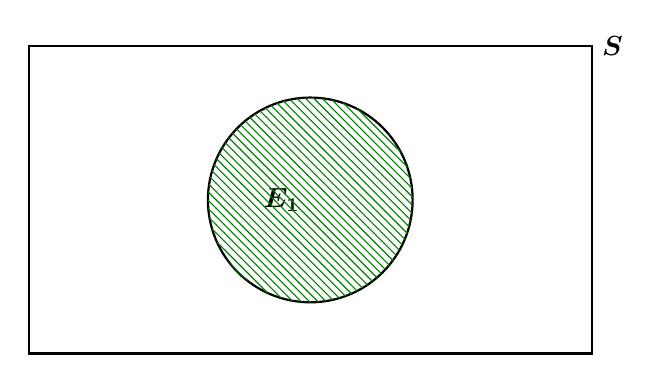
\begin{tikzpicture}[scale=.65]
      \visible<+->{\draw[thick]  (-4,-3) rectangle (7,3) node[anchor=north east, right] {$\bm S$};}
      \visible<+->{
        \draw[thick] (1.5,0) circle (2 cm) node[left] {$\bm{E_{1}}$};      
      }
      \visible<+->{
        \fill[pattern=north west lines,pattern color=green!50!black] (1.5,0) circle (2 cm);
      }
    \end{tikzpicture}      
  \end{center}
\end{block}


\end{frame}

\begin{frame}
  \frametitle{Basic axioms of probability (2)}

  \begin{block}{Axiom 2}
    The probability of a certain event $S$ is:
    \begin{equation}
      \label{eq:2}
      P(S) = 1
    \end{equation}
    \pause
    A certain event occupies the entire sample space

    \pause

    
    \begin{center}
      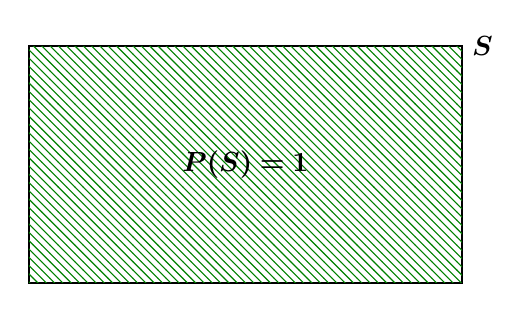
\begin{tikzpicture}[scale=.5]
        \visible<+->{\draw[thick]  (-4,-3) rectangle (7,3) node[anchor=north east, right] {$\bm S$};}
        \visible<+->{
          \fill[pattern=north west lines,pattern color=green!50!black](-4,-3) rectangle (7,3)  ;
        }
        \visible<+->{\node at (1.5,0) {$\bm{P(S) = 1}$};}
      \end{tikzpicture}      
    \end{center}
    \pause

    In other words, the probability of the sample space is unity (or 1).
  \end{block}

\end{frame}

\begin{frame}
  \frametitle{Basic axioms of probability (3)}
  \pause
  \begin{block}{Axiom 3}
    The probability of the union of $n$ mutually exclusive events is given by:

    \begin{equation}
      \label{eq:13}
      P(E_{1}\cup E_{2} \cup \cdots \cup E_{n}) = \pause P(E_{1}) + P(E_{2}) + \cdots + P(E_{n})
    \end{equation}
    \pause
    Equivalently,
    \pause
    
    \begin{equation}
      \label{eq:3}
      P\lt(\bigcup_{i=1}^n E_i\rt) = \sum_{i=1}^n P(E_i)
    \end{equation}

    \pause

    where:
    \begin{itemize}[<+->]
    \item $\bigcup_{i=1}^{n}$ denotes the union of sets (in this case, events $E_{i}$) indexed from $1$ through $n$     
    \item $\sum_{i=1}^{n}$ denotes the summation of quantities (in this case, probabilities $P(E_{i})$) indexed from $1$ through $n$
  \end{itemize}


  \end{block}
\end{frame}

\begin{frame}
  \frametitle{Example 1: Probability of mutually exclusive events}
  \pause

  If $E_{1}$ and $E_{2}$ are mutually exclusive events with probabilities $0.2$ and $0.3$, respectively.
  Find $P(E_{1}\cup E_{2})$.
  \pause
  
  \begin{center}
    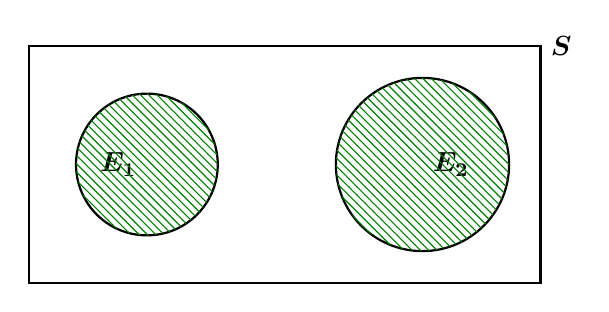
\begin{tikzpicture}[scale=.5]
      \visible<+->{\draw[thick]  (-5,-3) rectangle (8,3) node[anchor=north east, right] {$\bm S$};}
      \visible<+->{
        \draw[thick] (-2,0) circle (1.8 cm) node[left] {$\bm{E_{1}}$};
        \draw[thick]  (5,0) circle (2.2 cm) node[right] {$\bm{E_{2}}$};
      }
      \visible<+->{
        \fill[pattern=north west lines,pattern color=green!50!black] (-2,0) circle (1.8 cm);
        \fill[pattern=north west lines,pattern color=green!50!black](5,0) circle (2.2 cm);
      }
    \end{tikzpicture}      
  \end{center}

  \pause
  
  
  \begin{equation*}
    \label{eq:4}\gr
    P(E_1 \cup E_2) \pause = P(E_1) + P(E_2) \pause = 0.2 + 0.3 = \pause \boxed{0.5}
  \end{equation*}
  
\end{frame}

\begin{frame}
  \frametitle{Implications}

  \begin{itemize}[<+->]
  \item The probability of an event is always relative to that of others in the sample space

    \bigskip
    
  \item It is therefore convenient to normalize the probability of an event to that of its sample space (i.e. 1)

    \bigskip
    
  \item Thus

    \begin{equation}
      \label{eq:5}
      0\le P(E) \le 1
    \end{equation}

  \end{itemize}
\end{frame}

% \begin{frame}%<presentation:0>
%   \frametitle{Poll}
%   \pause
%   (This question tests your understanding of events and sample spaces.)
  
%   \begin{exampleblock}{}
%     Given an event $E$ in a sample space $S$ and that $P(E) = 0.2$.

%     \pause

%     \begin{enumerate}
%     \item Find the probability $P(E \cup S)$: \pause Answer: $E\cup S = S \pause \implies P(E\cup S) = P(S) = 1$
% \pause
%     \item Find the probability $P(\ol{E})$: \pause Answer: $P(\ol{E}) = 1 - P(E) = \pause 1 - 0.2 = 0.8$
%     \end{enumerate}
    
% \end{exampleblock}

% \end{frame}

\section{Addition Rule}
\begin{frame}
  \frametitle{The addition rule}

  Generally, the probability of the union of two events $E_1$ and $E_2$ is given by
  \pause
  
  \begin{equation}
    \label{eq:6}\bl
    P(E_1 \cup E_2) = P(E_1) + P(E_2) - P(E_1E_2)
  \end{equation}

  \pause

  Recall that $E_1E_2 \equiv E_1 \cap E_2$.\\

  \pause

  \bigskip

  The Venn diagram enables us to better visualize this.
  \pause

  \begin{center}
    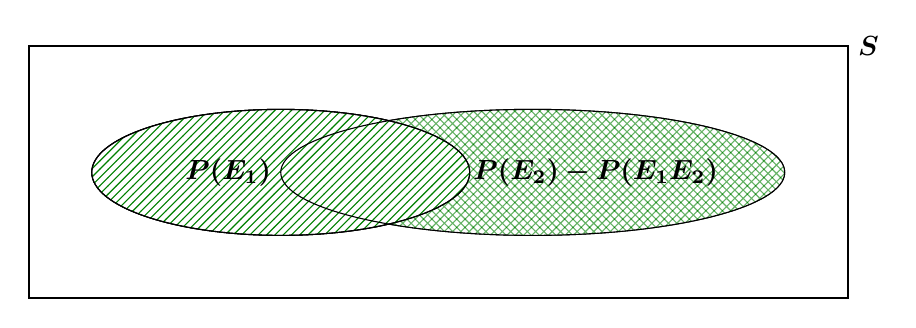
\begin{tikzpicture}[scale=.8]
      \visible<6->{\draw[thick]  (-5,-2) rectangle (8,2) node[anchor=north east, right] {$\bm S$};}
      \visible<7->{
        \draw[] (-1,0) ellipse (3 cm and 1 cm) node[left] {$\bm{E_{1}}$};
        \draw[]  (3,0) ellipse (4 cm and 1 cm) node[] {$\bm{E_{2}}$};
      }
      \visible<8->{
        \fill[white] (-1,0) ellipse (3 cm and 1 cm) ;
        \fill[white] (3,0) ellipse (4 cm and 1 cm) ;
        \fill[draw,pattern=north east lines,pattern color=green!50!black]
        (-1,0) ellipse (3 cm and 1 cm) node[left] {$\bm{P(E_{1})}$};
      }

      
      \visible<9->{        
        \begin{scope}[even odd rule]
          \clip (3,0) ellipse (4 cm and 1 cm);
          \fill[pattern=crosshatch, pattern color=green!50!black, opacity=.6] 
          (-1,0) ellipse (3 cm and 1 cm)
          (-5,-2) rectangle (8,2) ;
          \node at (4,0)  {$\bm{P(E_{2}) -  P(E_{1}E_{2})}$};
        \end{scope}
        \draw[] (-1,0) ellipse (3 cm and 1 cm) ;
        \draw[]  (3,0) ellipse (4 cm and 1 cm);
      }


    \end{tikzpicture}
  \end{center}  
\end{frame}



\begin{frame}
  \frametitle{Addition rule for mutually exclusive events}
  \pause

  Recall: given two events $E_1$ and $E_2$:
  \pause
  
  \begin{equation}
    \label{eq:6}
    P(E_1 \cup E_2) = P(E_1) + P(E_2) - P(E_1E_2)
  \end{equation}
  
  If the events  $E_1$ and $E_2$, are mutually exclusive, then

  \pause

  \begin{equation*}
    P(E_{1}E_{2}) = 0
  \end{equation*}
  \pause

  Thus,
  
  \begin{equation}
    \label{eq:7}
    P(E_1 \cup E_2) = P(E_1) + P(E_2) - 0 
  \end{equation}
  \pause

  which yields Axiom 3.

\end{frame}


\begin{frame}
  \frametitle{Complementary events}
  \pause

  Recall that the union of an event and its complement yields the entire sample space: \pause
  \begin{equation}
    \label{eq:8}
    E \cup \overline{E} = S
  \end{equation}
  \pause
  
  Thus, we have
  \begin{equation}
    \label{eq:9}
    P(E\cup \ol{E}) = P(S) = \pause 1
  \end{equation}

  \pause

  Given that $E$ and $\ol{E}$ are also mutually exclusive, from Eq.\ \ref{eq:7} we obtain: \pause
  \begin{eqnarray}
    \label{eq:10}
    P(E\cup \ol{E}) &=& P(E) + P(\ol{E}) = 1 \\ \pause
      \therefore \alert{ P(\ol{E})} &=& \alert{ 1 - P(E) }
  \end{eqnarray}
  \pause

  Equivalently, $P(E) = 1 - P(\ol{E})$.\pause \alert{\quad \it Complement Rule}
\end{frame}



\begin{frame}
  \frametitle{Example 2: Left-turn lane design}
  60 observations of the number of vehicles waiting for left turns at an intersection are shown in the table.
  \pause

      \begin{center}
      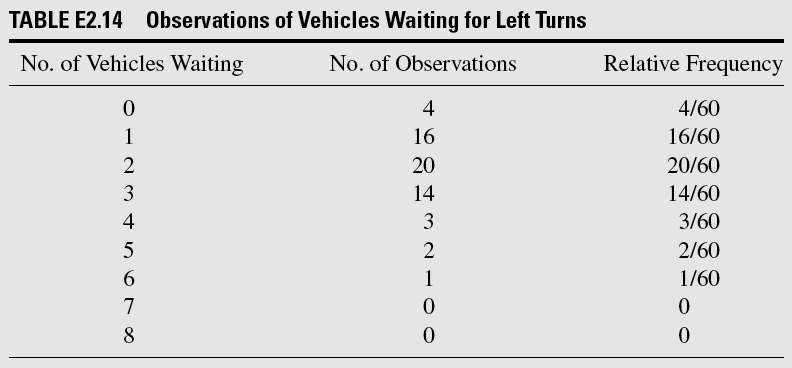
\includegraphics[width=.5\textwidth, trim={0 0 0 1.2cm},clip]{E_02_14_tbl} 
    \end{center}

    \pause
    
  Given the following definitions:
    \begin{align*}
      E_1 &= \text{$>$ 2 vehicles waiting for left turns} \\ 
      E_2 &= \text{$\le$ 4 vehicles waiting for left turns}
    \end{align*}
    \pause    
    Find the following probabilities: 

  
    \pause
    \begin{enumerate}[(a)]
    \item $P(E_1)$
    \item $P(E_2)$
    \item $P(E_1E_2)$
    \item $P(E_1 \cup E_2)$
    \end{enumerate}
 \end{frame}



\begin{frame}
  \frametitle{Example 2: Left-turn lane design (cont.)}

        \begin{center}
      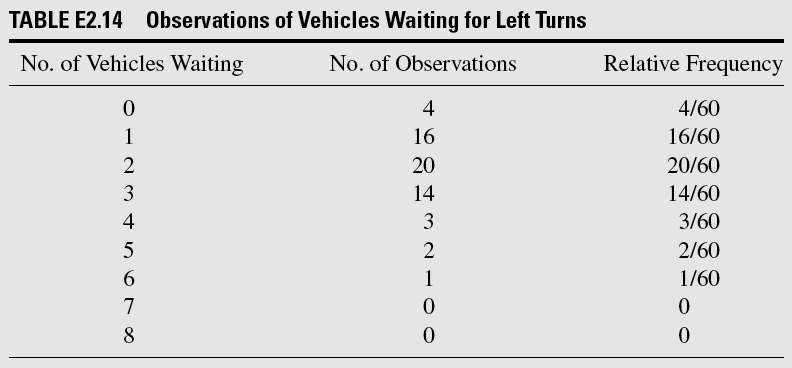
\includegraphics[width=.5\textwidth, trim={0 0 0 1.2cm},clip]{E_02_14_tbl} 
    \end{center}
    
    \pause

    Let $X$ be the number of vehicles. \pause
    
    \begin{enumerate}[(a)]
    \item $P(E_1) = \pause
      P(X > 2) = \pause
      1 - P(\ol{E_1}) = 1 - \fr4{60} - \fr{16}{60} - \fr{20}{60} = \fr{20}{60}$ \pause \\

      \medskip

    \item $P(E_2) = \pause
      P(X \le 4) =  \pause \fr{4}{60} + \fr{16}{60} + \fr{20}{60} + \fr{14}{60} +
      \fr{3}{60}= \fr{57}{60}$ \pause \\

      \medskip
      
    \item $P(E_1E_2) = \pause
      P(X >2 \text{ and } X \le 4) = \pause
      P(2 < X \le 4) $ \\[2mm] \pause
      $= P(X=3) + P(X=4) = \pause \fr{14}{60} + \fr{3}{60} = \fr{17}{60}$ \pause \\

      \medskip
      
    \item $P(E_1 \cup E_2) \pause  = P(E_1) + P(E_2) - P(E_1E_2) \pause  = \fr{20+57-17}{60} = \pause 1$ 
    \end{enumerate}
    \pause
    How would you characterize $E_1$ and $E_2$?
    \pause \quad \framebox{\alert{Collectively exhaustive events}}

\end{frame}



\section{Counting methods}

\begin{frame}
  \frametitle{Fundamental principle of counting}
  \pause

  Given $1, 2, \ldots, k$ operations are to be performed, and $n_{1}, n_{2}, \ldots, n_{k}$
  ways of performing each respective operation.
  \pause

  \bigskip

  The total number of possibilities is given by

  \begin{equation*}
    n_{1} \times n_{2} \times \cdots \times n_{k}
  \end{equation*}

\end{frame}


\begin{frame}
  \frametitle{Example 3: Ice cream store}
    \pause

    An ice cream store has the following options for an order (only one size is available):

    \bigskip
    
    \pause

    \begin{minipage}{.25\linewidth}
      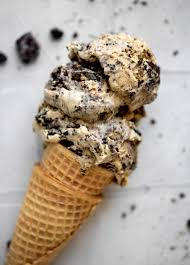
\includegraphics[width=.6\textwidth]{ice}
    \end{minipage}\quad
    \begin{minipage}{.7\linewidth}
    \begin{itemize}[<+->]
    \item Three types of cone (cups are not available)
    \item Ten flavors
    \item Four toppings (which cannot be combined)
    \end{itemize}
  \end{minipage}

  \pause

  \bigskip
    How many distinct ice cream orders are possible? \pause

    \[ \gr 3 \times 10 \times (4 + 1) = \boxed{150}\]

    (Note: you can order an ice cream without any topping, hence 5 topping possibilities
\end{frame}

\begin{frame}%<presentation:0>
  \frametitle{Example 4: License plate numbers}
  \pause

  A certain state uses only digits (including ``0'') for its license plate numbers. \pause

  \begin{center}
    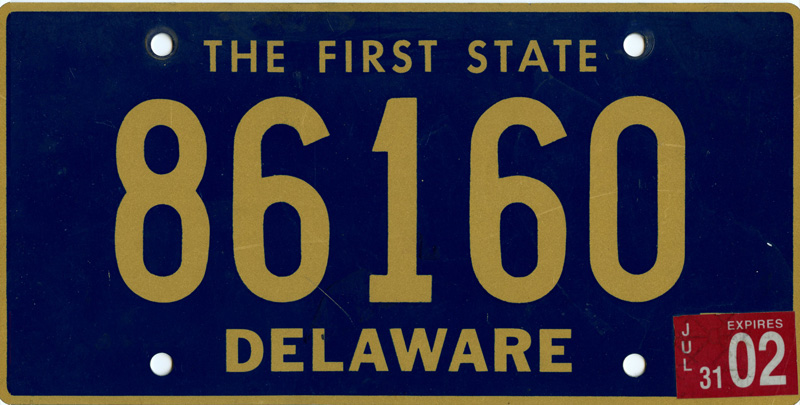
\includegraphics[width=.3\textwidth]{delaware}
  \end{center}
  
  If every number must have 5 digits, how many distinct license plate numbers are available? \pause

  \begin{exampleblock}{}
    There are 10 digits ($0,1 , \ldots, 9$).\\
    
    \pause
    
    The number of possible license plates is thus given by \pause

    \begin{equation*}
      10 \times 10 \times 10 \times 10 \times 10   =\pause 10^{5}
    \end{equation*}
  \end{exampleblock}
  \pause

  If in 2021, the state releases a new series of plate numbers that must now end with a letter in
  addition to 5 preceding digits, how many distinct plates can be manufactured? \pause  Answer: $\gr 26 \times 10^{5} = 2,600,000$
\end{frame}

\begin{frame}
  \frametitle{Permutations}\pause

  A permutation is an arrangement (ordering) of objects in a collection.

  \pause
  
  \begin{block}{Definition} \pause
  The number of permutations of $n$ objects is given by $n!$ (pronounced ``$n$ factorial''), where

  \pause
  \begin{equation}
    \label{eq:10}
    n! = n \times (n-1) \times (n-2) \times \cdots \times 2 \times 1
  \end{equation}
\end{block}
  \pause

  \begin{exampleblock}{Examples of factorials}\pause
    \begin{itemize}
    \item $2! = \pause 2\times 1 = 2$\pause
    \item $3! = \pause 3\times 2 \times1 = \pause 6$\pause
    \item $4! = 4 \times 3 \times 2 \times 1 = \pause 24$ \pause
    \item $5! = \pause 5 \times 4! = \pause 120$ \pause
    \item $0! = 1$
    \end{itemize}
  \end{exampleblock}
\end{frame}

\begin{frame}
  \frametitle{Example 5: Ordering numbers}
  \pause
  In how many ways can 3 rag dolls be arranged in a row? \pause

  \bigskip
  
  \begin{center}
    
\begin{tikzpicture}
      {\bl \Strichmaxerl[2]}      
    \end{tikzpicture}\qquad
    
\begin{tikzpicture}
      {\gr \Strichmaxerl[2]}      
    \end{tikzpicture}\qquad
    
\begin{tikzpicture}
      {\rd \Strichmaxerl[2]}      
    \end{tikzpicture}  
  \end{center}

  \pause

  \begin{exampleblock}{}
    The number of possibilities is given by:\pause
    
    \begin{equation*}
      3! = 3 \times 2 \times 1 = \pause 6
    \end{equation*}
    \pause
    Let's count them: \pause


\begin{minipage}{.45\linewidth}
  
\end{minipage}
\begin{minipage}{.5\linewidth}
  \bigskip
    \begin{enumerate}[<+->]
    \item 
\begin{tikzpicture}      {\bl \Strichmaxerl[2]}      
      \end{tikzpicture}\qquad
      
\begin{tikzpicture}
        {\gr \Strichmaxerl[2]}      
      \end{tikzpicture}\qquad
      
\begin{tikzpicture}
        {\rd \Strichmaxerl[2]}      
      \end{tikzpicture}

    \item 
\begin{tikzpicture}      {\bl \Strichmaxerl[2]}      
      \end{tikzpicture}\qquad
      
\begin{tikzpicture}
        {\rd \Strichmaxerl[2]}      
      \end{tikzpicture}\qquad
      
\begin{tikzpicture}
        {\gr \Strichmaxerl[2]}      
      \end{tikzpicture}

    \item
\begin{tikzpicture}{\gr \Strichmaxerl[2]}      
      \end{tikzpicture}\qquad
      
\begin{tikzpicture}
        {\bl \Strichmaxerl[2]}      
      \end{tikzpicture}\qquad
      
\begin{tikzpicture}
        {\rd \Strichmaxerl[2]}      
      \end{tikzpicture}


    \item 
\begin{tikzpicture}{\gr \Strichmaxerl[2]}      
      \end{tikzpicture}\qquad
      
\begin{tikzpicture}
        {\rd \Strichmaxerl[2]}      
      \end{tikzpicture}\qquad
      
\begin{tikzpicture}
        {\bl \Strichmaxerl[2]}      
      \end{tikzpicture}


    \item 
\begin{tikzpicture}{\rd \Strichmaxerl[2]}      
      \end{tikzpicture}\qquad
      
\begin{tikzpicture}
        {\bl \Strichmaxerl[2]}      
      \end{tikzpicture}\qquad
      
\begin{tikzpicture}
        {\gr \Strichmaxerl[2]}      
      \end{tikzpicture}

    \item 
\begin{tikzpicture}      {\rd \Strichmaxerl[2]}      
      \end{tikzpicture}\qquad
      
\begin{tikzpicture}
        {\gr \Strichmaxerl[2]}      
      \end{tikzpicture}\qquad
      
\begin{tikzpicture}
        {\bl \Strichmaxerl[2]}      
      \end{tikzpicture}



    \end{enumerate}
  \end{minipage}

  \end{exampleblock}
\end{frame}

\begin{frame}
  \frametitle{Permutations of a subset}
  \pause

  The number of ways $n$ objects can be arranged is $n!$ \pause

  \bigskip

  However, if a subset of $k$ objects is chosen from a set of $n$ objects, the number of permutations (ways of choosing and arranging) of this subset is given by \pause

  \begin{equation}
    \fr{n!}{(n-k)!}
  \end{equation}


\end{frame}


\begin{frame}
  \frametitle{Example 6: 3-letter license plates}\pause
    In a small state, plate numbers must have only 3 non-repeating characters (letters). How many permutations are there?
    \pause

    \bigskip
    
    \begin{enumerate}[Method 1.]
    \item There are 26 possibilities for the first character. \pause
      After this, 25 options are left for the second character, \pause
      and then 24 for the third. The permutations are thus: \pause
      $\gr\boxed{26\times 25 \times 24 = 15600}$
      \pause

      \bigskip
      
    \item We can use the formula for the permutations of a subset of $k$ items from a set of $n$: \pause
\gr
      \begin{eqnarray*}
        \fr{n!}{(n-k)!} &=& \fr{26!}{(26-3)!}\pause = \fr{26!}{(23)!}  \\\pause
                        &=& \fr{26 \times 25 \times 24 \times \cancelto<11->{1}{23!}}{
                            \cancelto<11->{1}{23!}} \pause \\\pause
                        &=& 26 (25)(24) = \pause 15600                            
      \end{eqnarray*}
      
    \end{enumerate}
  \end{frame}

\begin{frame}
  \frametitle{Permutations with repetition}
  \pause

  Without repetition, the number of permutations of $n$ objecst is $n!$.

  \bigskip

  However, if there are $n_{1}$ identical (or repeated) items of type 1, $n_{2}$ identical items of type 2, \dots,
  and $n_{k}$ identical items of type $k$, then the number of permutations is given by

  \begin{equation}
    \fr{n!}{n_{1}!n_{2}!\times \cdots \times n_{k}!}
  \end{equation}

  
  \begin{exampleblock}{How many ways can the letters in the word ``MASS'' be arranged?}
    

    The letter ``S'' is repeated. Thus, the number of permutations are:

    \begin{equation*}
      \fr{4!}{2!} = 4 \times 3 = 12
    \end{equation*}

    %You may verify this in MATLAB using the \texttt{perms} function.
  \end{exampleblock}
    
\end{frame}

\begin{frame}
  \frametitle{Combinations}
  \pause

  A combination is distinct subset of objects selected from a collection. \pause

  \bigskip
  
  \begin{block}{Definition}\pause
  The number of possible combinations of $k$ objects chosen from a collection of $n$ objects is given by
  ${n \choose k}$ (pronounced ``$n$ choose $k$''):\pause

  \begin{equation}
    \label{eq:11}
    {n\choose k} = \fr{n!}{k!(n-k)!}
  \end{equation}

  
\end{block}
\pause

\bigskip

With combinations, the order is not important (in constrast to permutations).

\end{frame}

\begin{frame}
  \frametitle{Example 7: Choosing a basketball team}
  \pause

  You need to form a basketball team of five. You have a group of 8 players to choose from.
  How many different teams can you form? \pause

  \begin{exampleblock}{}
    The number of combinations is given by\pause

    \begin{eqnarray*}
      {8 \choose 5} &=& \fr{8!}{5!(8-5)!} = \pause \fr{8!}{5!3!} \\ \pause
                    &=& \fr{8 \times 7 \times 6 \times \cancelto<7->{1}{5!}}
                        {\cancelto<7->{1}{5!}\cdot 3!} \\\pause\pause
                    &=& \fr{8(7)(6)}{3(2)(1)} \pause = \boxed{56}
    \end{eqnarray*}

    \pause

    You can form 56 different teams.
  \end{exampleblock}
  
  
\end{frame}




\section{Outlook}
\begin{frame}
  \frametitle{Recap}\pause
  \begin{itemize}[<+->]
  \item Three {\gr \bf axioms} of probability:\pause
    \begin{eqnarray*}
     \text{\gr Ax. 1: } \pause P(E) &\ge& 0 \quad \text{and} \quad P(E) \le 1 \\\pause
     \text{\gr Ax. 2: } \pause P(S) &=& 1 \\\pause
     \text{\gr Ax. 3: } \pause P(E_{1}\cup E_{2}\cup \cdots\cup E_{n}) &=& P(E_{1}) + P(E_{2}) + \cdots + P(E_{n})
    \end{eqnarray*} \pause
  \item Addition rule: $P(A\cup B) = P(A) + P(B) - P(AB)$
    \begin{itemize}
      \item For {\rd mutually exclusive} events: $P(A\cup B) = P(A) + P(B)$ \quad (Axiom 3)
    \end{itemize}
  \item Counting
    \begin{itemize}[<+->]
    \item \textbf{Fundamental principle} of counting: number of outcomes for $1, \ldots, k$ events, each with $n_{1},\ldots, n_{k}$ possibilities is \pause  $n_{1}\times\cdots \times n_{k}$
    \item \textbf{Permutations}  (arrangements) of $n$ objects: $n! = n(n-1)(n-2)\cdots(2)(1)$
    \item Permutations of a \textbf{subset} of $k$ items chosen from set of $n$ items: $n!/(n-k)!$
    \item \textbf{Combinations} (distinct; order not important) of group of $k$ items chosen from set of $n$ items: $n!/(k!(n-k)!)$
    \end{itemize}
  \end{itemize}
\end{frame}
 



%\backupbegin
\section{Appendix}


\begin{frame}
  \frametitle{The addition rule: three events}

  The probability of the union of three events is given by \pause

  \begin{align}
    \label{eq:6b}
    \begin{split}
      P(E_1 \cup E_2 \cup E_3) &= P[(E_1 \cup E_2) \cup E_3] \\  
      &= {\bl P(E_1 \cup E_2)} + P(E_3) - {\gr P[(E_1\cup E_2)E_3]}  \quad \text{\og addition rule} \\  
      &= {\bl P(E_1) + P(E_2) - P(E_1E_2)} + P(E_3) \\
      &  \qquad - {\gr [ P(E_1E_3 \cup E_2E_3)\gr} \pause \quad \text{\og addition rule; distributive} \\  
      &= {\bl P(E_1) + P(E_2) - P(E_1E_2)} + P(E_3) \\
      &  \qquad- {\gr [ P(E_1E_3)  + P(E_2E_3) - P(E_1E_3E_2E_3)} \\  
      &= P(E_1) + P(E_2) - P(E_1E_2) + P(E_3) \\
      &\qquad - P(E_1E_3)  - P(E_2E_3) + P(E_1E_2E_3)   \\  
      \therefore \bm { P(E_1 \cup E_2 \cup E_3)} & \bm{=  P(E_1) + P(E_2) + P(E_3)} \\
       & \qquad \bm{- P(E_1E_2) - P(E_1E_3)  - P(E_2E_3) + P(E_1E_2E_3)}
    \end{split}
  \end{align}
\end{frame}


\begin{frame}
  \frametitle{Complementary events (cont.)}
  \pause
  What if we want to find the probability of the union of multiple events?
  \pause

  \bigskip
  \begin{equation}
    P(E_1 \cup E_2 \cup \cdots E_n) = 1 - P(\ol{E_1\cup E_2 \cup \cdots \cup E_n})
  \end{equation}
  
  \pause

  {\og How would we simplify the right-hand side?} \pause

    Apply de Morgan's rule:  \pause

  \begin{equation}
    \therefore  P(E_1 \cup E_2 \cup \cdots E_n) = 1 - P(\ol{E_1}\,\ol{E_2}\cdots\ol{E_n})
  \end{equation}

\end{frame}


%\backupend

%\begin{frame}[allowframebreaks]
%   \frametitle{References}
%   \AtNextBibliography{\scriptsize}
%   \setbeamertemplate{bibliography item}[text]
%   \printbibliography[heading=none]
  
% \end{frame}

%\printbibliography
\end{document}
%%% Local Variables:
%%% mode: latex
%%% TeX-master: t
%%% End:
